\subsection{Vinkelberegning}\label{sec:imp_vinkler}
I \autoref{sec:test_acc} fremgår det, at der er lineær sammenhæng mellem vinklerne over tid. Det er derfor muligt at udføre en lineær interpolation over dataen af målinger fra accelerometrene i forskellige vinkler. På denne måde er det muligt at bestemme, hvilken som helst vinkel for en tilsvarende spænding. Da målingerne af linearitet, målt i \autoref{sec:test_acc}, er foretaget med Ni USB-6009 stemmer spændingerne ikke overens, når det samples på mikrokontrolleren. Derfor udføres der en ny måling af linearitet med mikrokontrolleren, hvor spændingen i de forskellige vinkler er målt. Efterfølgende er der aflæst et offset, som er trukket fra, for at centrere signalet omkring 0. Offsettet for accelerometeret placeret på låret er aflæst til $-1003~V$ og accelerometeret placeret på skinnebenet til $-972~V$. De målte spændinger, hvor signalet er offsetjusteret fremgår af \autoref{tab:vinkelinterval_psoc}. .

%\begin{comment}
%\begin{table}[H]
%	\centering
%	\begin{tabular}{|l|l|l|}
%				%& \textit{Accelerometer placeret på låret} &				
%	\textbf{Interval} & \textbf{Målt spænding} & \textbf{Målt spænding} 	\\ \hline	
%    \textbf{0-10} 			& $0~V$							& $-186~V$   \\ \hline
%    \textbf{10-30} 			& $-31~V$						& $-185~V$	\\ \hline
%    \textbf{30-50} 			& $-67~V$						& $-168~V$	\\ \hline
%    \textbf{50-70} 			& $-126~V$						& $-126~V$	\\ \hline
%    \textbf{70-80} 			& $-168~V$						& $-67~V$	\\ \hline
%    \textbf{80-90} 			& $-185~V$						& $-31~V$	\\ \hline
%    				%& \textit{Accelerometer placeret på skinnebenet} &		
%    	\textbf{Interval} & \textbf{Målt spænding} & \textbf{Målt spænding} 		\\ \hline	
%    \textbf{0-10}			& $0~V$ 							& $-179~V$	    \\ \hline
%    \textbf{10-30}			& $-16~V$						& $-176~V$	 	\\ \hline
%    \textbf{30-50}			& $-52~V$						& $-153~V$		\\ \hline
%    \textbf{50-70}			& $-111~V$						& $-111~V$		\\ \hline
%    \textbf{70-80}			& $-153~V$						& $-52~V$	 	\\ \hline
%     \textbf{80-90}			& $-176~V$						& $-16~V$	 	\\ \hline
%	\end{tabular}
%	\caption{Spændingen målt i vinklerne fra 0 til 90$^{\circ}$ for accelerometrene placeret på både låret og skinnebenet. Den første spænding svarer til start intervallet og den sidste til slutningen afintervallet.}
%	\label{tab:vinkelinterval_psoc}
%\end{table}
%\end{comment}


\begin{table}[]
\centering
\begin{tabular}{lcc}
         & \textit{Accelerometer placeret på låret}                           & \multicolumn{1}{l}{}                      \\ \hline
Interval & Målt spænding {[}V{]}                                              & \multicolumn{1}{l}{Målt spænding {[}V{]}} \\ \hline
0 - 10   & 0                                                                  & - 31                                      \\ \hline
10 - 30  & - 31                                                               & - 67                                      \\ \hline
30 - 50  & - 67                                                               & - 126                                     \\ \hline
50 - 70  & - 126                                                              & - 168                                     \\ \hline
70 - 80  & - 168                                                              & - 185                                     \\
\hline
80 - 90  & -185                                                               & - 186                                     \\
\hline
         & \multicolumn{1}{l}{\textit{Accelerometer placeret på skinnebenet}} & \multicolumn{1}{l}{}                      \\ \hline
Interval & Målt spænding {[}V{]}                                              & \multicolumn{1}{l}{Målt spænding {[}V{]}} \\ \hline
0 - 10   & 0                                                                  & - 16                                      \\
\hline
10 - 30  & - 16                                                               & - 52                                      \\
\hline
30 - 50  & - 52                                                               & - 111                                     \\
\hline
50 - 70  & - 111                                                              & - 153                                     \\
\hline
70 - 80  & - 153                                                              & - 176                                     \\
\hline
80 - 90  & - 176                                                              & - 179    \\ \hline 
\end{tabular}
\caption{Spændingen målt i vinklerne fra 0 til 90$^{\circ}$ for accelerometrene placeret på både låret og skinnebenet. Den første spænding svarer til start intervallet og den sidste til slutningen afintervallet.}
\label{tab:vinkelinterval_psoc}        
\end{table}

Spændingen er målt for vinklerne fra 0 til 90$^{\circ}$ for accelerometrene placeret på både låret og skinnebenet. Den første målte spænding er for startværdien i intervallet og den sidste spænding er slutværdien i intervallet.

Ud fra de målte værdier i de forskellige intervaller, er der opstillet en funktion indeholdt ifelse-løkker, hvorved det er muligt at vurdere, hvilket interval en given spænding befinder sig i. I hver enkelt løkke anvendes lineær interpolation, som har til opgave at finde en vinkel, der er svarende til en spænding som ligger mellem intervallet og returnerer denne. 

Når der er udført lineær interpolation over dataen skal de målte data fra låret samt skinnebenet ligges sammen for at få den samlede vinkel af, hvor langt personen har bevæget sig, og derved befinder sig i squat-øvelsen. Resultaterne er optaget på mikrokontrolleren og visualiseres i MATLAB, hvilket fremgår af \autoref{fig:acc_imp}.
 

\begin{figure}[H]
\centering
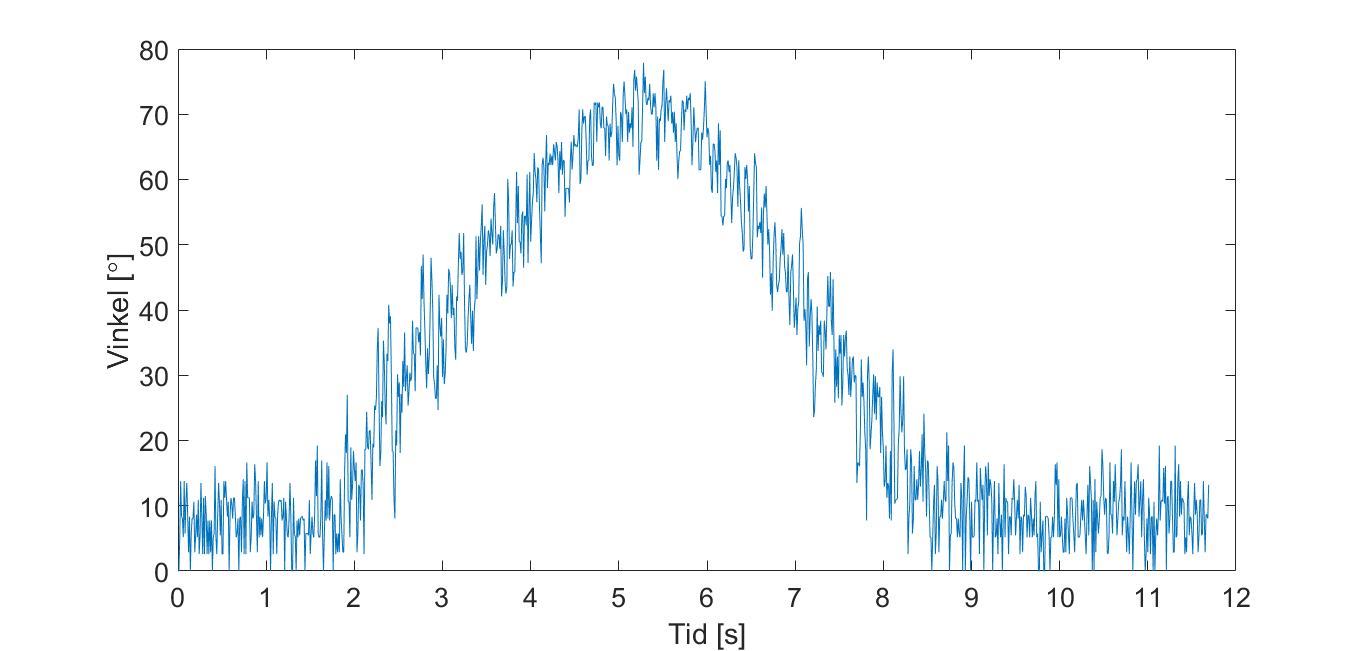
\includegraphics[width=0.8\textwidth]{figures/Pilotforsoeg/accvinkel}
\caption{Samlet vinkler af accelerometrene under udførelse af squat-øvelsen}
\label{fig:acc_imp}
\end{figure}



